\documentclass[12pt]{article}

% Load packages
\usepackage[top=1in, bottom=1in, left=1in, right=1in]{geometry}
\usepackage{graphics}
\usepackage[pdftex]{graphicx}
\usepackage{epsfig}
\usepackage{epsf}
\usepackage{epstopdf}
\usepackage{mathrsfs}
\usepackage{amsmath}
\usepackage{amssymb}
\usepackage{textcomp}
\usepackage[scaled=.90]{helvet} % Helvetica (currently not used)
\usepackage[]{lineno} % For line numbers
\usepackage{natbib}
\usepackage{sidecap}

% Define new commands and definitions
\def\ds{\displaystyle}
\def\d{\partial}
\newcommand{\rr}{\mathbb{R}}
\newcommand{\zz}{\mathbb{Z}}
\newcommand{\nn}{\mathbb{N}}
\newcommand{\ee}{\mathscr{E}}
\newcommand{\mb}{\mathbf}
\newcommand{\ol}{\overline}

% Text formatting
\linespread 2	
\linenumbers

\title{Escape direction does not matter for some fish prey}

\author{Alberto Soto, William J. Stewart and Matthew J. McHenry\\
  Department of Ecology \& Evolutionary Biology,\\
  University of California, Irvine\\ \\ \\ \\}



%\date{}                                           % Activate to display a given date or no date

\begin{document}
\DeclareGraphicsExtensions{.eps,.pdf,.png,.gif,.jpg,.ps}

\maketitle

\pagebreak


% ABSTRACT
% --------------------------------------------------------------------------------
\begin{abstract}

Predator-prey interactions in fish are commonly studied with an interest in determining whether prey adopt an optimal strategy to evade predators. However, it is not clear under what circumstances an optimal strategy aids a prey's survival. Here we examine the theoretical consequences of deviation from optimal strategy for predators that approach at different speeds. With a focus on the minimum distance between predator and prey, we simulated these interactions with numerical and analytical mathematics and compared our predictions with measurements in zebrafish (\textit{Danio rerio}). We found that differences in escape direction had only a small effect on the minimum distance when predators were more than an order of magnitude faster than the prey. Furthermore, differences in direction had no effect on performance for a broad range of escape angles when the prey were faster than the predator, which is the case for zebrafish. Therefore, the escape angle either has no optimum or has a minor effect on predator-prey interactions in many situations where the predator is either slower or much faster than the prey. Optimal strategy is therefore most meaningful when prey are approached by a predator of intermediate speed. It remains to be seen whether prey behave optimally in this domain or whether optimal responses serve to enhance survivorship.

\end{abstract}

\pagebreak

%TODO:Cite Holzmann SIFF paper

% --------------------------------------------------------------------------------
\section{Introduction}
\label{intro}

Biologists have long--appreciated the importance of predation in the ecology and evolution of prey species. This subject is extensive enough to fill the pages of books with the fascinating diversity of strategies that prey use to avoid encounters with predators \citep[e.g.][]{Ruxton:2004vb} or to defend themselves when discovered \citep[e.g.][]{Emlen:2014wb, Evans:1990va}. In contrast, our understanding for how prey evade capture by locomotion is relatively rudimentary. Although biomechanical studies commonly speculate on the importance of locomotor performance to survival, relatively few have tested what aspects of locomotion are most meaningful in these interactions. Studies that have explored this subject \citep[reviewed by][]{Domenici:2011tv} underscore the common-sense notion that the direction of an escape matters to a prey's survival. This idea is formalized by pursuit models that aim to determine the optimal direction of an escape response. The present study examined such a model \citep{Weihs:1984tb} to consider the strategic consequences of deviating from optimal strategy in piscivorous interactions. We compare the predictions of this model to experimental results in zebrafish (\textit{Danio rerio}) \citep{Stewart:2014cm} and offer new interpretations of theory on prey strategy.

Pursuit models are an area of game theory that offers a basis for examining locomotor behavior in strategic terms. There is recent interest in revisiting these models \citep[e.g.][]{Howland:1974, Weihs:1984tb} with experimental studies that consider the behavior of both predators and prey. This includes work on running vertebrates \citep[e.g.][]{Wilson:2014fd}, birds \citep[e.g.][]{Hedenstrom:2001do, Kullberg:1998ur} and bats \citep[e.g.][]{Ghose:2006dk} in flight, running insects \citep{Domenici:2008kra}, flying insects \citep[e.g.][]{Combes:2012eta}, and swimming zooplankton \citep[e.g.][]{Arnott:1999wx, Heuch:2007kk} and fishes \citep[e.g.][]{Domenici:2000un}. These efforts offer the potential to reveal how sensory and motor systems govern the outcome of predator--prey interactions. 

A piscivorous interaction offers some advantages as a model for examining the sensory-motor basis of predator evasion. In many cases, this interaction can be easily studied in a laboratory. Under artificial conditions, predatory fishes attempt to feed on prey and prey initiate a `fast-start' escape response (Fig. \ref{pred_prey}). Both players operate with motion that is largely two-dimensional and therefore relatively simple to measure and describe. Zebrafish exhibit both predator evasion and predatory behavior in the lab \citep{Stewart:2013bh} and this species offers a growing wealth of understanding in physiology and neuroscience \citep[e.g.][]{McLean:2011gi, Briggs:2002uf} that may be leveraged for mechanistic insight on predator--prey interactions. In addition, fish offer one of the few biological pursuit systems that have been mathematically modeled \citep{Weihs:1984tb}. This model offers specific predictions of swimming trajectories that may be tested with kinematic measurements. 

Deviation from optimal strategy has commonly been interpreted as a strategic adaptation. The protean hypothesis suggests that prey which are unpredictable should have an advantage in predator evasion over predictable prey \citep{Humphries:1970hy}. This idea may apply to the erratic motion of an individual or to predators that learn or adapt to the behavior of a population of prey that exhibits variable motion. The 'fast start' escape response of fish generates a turn and acceleration of the body in a particular direction and therefore would appear to correspond to the latter category \citep{D:1973up}, although a sequence of fast starts could offer the opportunity for erratic motion. Nonetheless, a potential trade-off exists for the direction of a fast start between optimal displacement away from an advancing predator and the benefit of being unpredictable.  

Interpretations of prey motion have generally not considered the effect of deviating from optimal strategy. For example, it is not clear whether an escape that is 5\textdegree\hspace{0.5pt} or 50\textdegree\hspace{0.5pt} from the optimum predicted by Weihs and Webb (1984) has a major or negligible effect on evasion success. If evasive performance is insensitive to differences in escape direction, then no trade-off exists between evasiveness and predictability. In short, it is unclear when optimal strategy matters. The present study therefore revisited the mathematics of the Weihs and Webb (1984) model to examine how deviation from optimal strategy affects prey evasion. We expanded this model and performed numerical simulations for comparison with experimental results. In this effort, we arrived at new interpretations of theory on prey evasion. In particular, we identified conditions where the escape direction is predicted to have little or no effect on the evasiveness of prey.

% --------------------------------------------------------------------------------
\section{Optimal prey strategy}
\label{opt_strategy}

The Homicidal Chauffeur is the colorful title for a pursuit game that has been applied to a variety of systems, including predator--prey interactions \citep{Isaacs:1965va}. Pursuit games consider the trajectories of its players and thereby address the effects of directional decision--making to the outcome of an interaction. Weihs and Webb (1984) adopted the Homicidal Chauffeur to model the responses of a prey fish that encounters a predator fish. Here we offer a brief review of this model as a means to explain the basis for our expansion of the theory and our interpretations of prey strategy, though a more complete derivation is presented in the original study \citep{Weihs:1984tb}.

The payoff is a quantity used in game models to define the beneficial or detrimental consequences of playing with a particular strategy \citep{Webb:2007hg}. For pursuit models, the payoff is often defined as the minimum distance between predator and prey. This quantity reflects the condition where the predator has the best opportunity to capture the prey. The optimal strategy for an evasive prey is therefore defined as the escape angle that yields the greatest minimum distance (Weihs and Webb, 1984).

Predicting the distance between predator and prey requires relatively few parameters under some simplifying assumptions. In the rapid events of a predatory strike, it is reasonable to approximate the predator's motion as a constant speed, $U$. If one neglects the acceleration period of the fast start, then the prey's motion may be approximated with a constant speed, $V$, at an escape angle $\alpha$, defined with respect to the heading of the predator (Fig. \ref{pred_prey}A). Under these conditions, the distance between predator and prey, $D$, may be calculated over time:
%
\begin{equation}
D^2 = ((X_0 - Ut) + Vt\cos\alpha)^2 + (Vt\sin\alpha)^2,
\label{dist}
\end{equation}
%
where $X_0$ is the starting position of the prey.

The minimum distance, the payoff in this game, may be calculated from the distance equation. The first step is to calculate the time, $t_{\text{min}}$,  at which the minimum distance occurs. This may be found from the root of the first derivative of Eqn. \ref{dist} with respect to time, which yields the following solution:
%
\begin{equation}
t_{\text{min}} = \frac{X_0}{V} \frac{K-\cos\alpha}{1-2 K\cos\alpha+K^2},
\label{eq33weihs}	
\end{equation}
%
where $K$ indicates the speed of the predator relative to the prey ($K = U/V$). Weihs and Webb observed that this equation yields negative values of time where $K<1$ and is therefore only useful when the predator is faster than the prey (Weihs and Webb, 1984). The minimum distance was consequently determined for $K>1$ by solving for distance (Eqn. \ref{dist}) at $t_{\text{min}}$:
%
\begin{equation}
\ol D_{\text{min}}^2 = \frac{D_{\text{min}}^2}{X_0^2} = \frac{\sin^2\alpha}{K^2 - 2K \cos\alpha + 1},
\label{dmin}
\end{equation}
where $\ol D_{\text{min}}$ is the minimum distance normalized by the starting position of the prey.

Finally, the optimal strategy for the prey may be determined by finding the escape angle that yields the greatest minimum distance. This occurs where the derivative of Eqn. \ref{dmin} with respect to $\alpha$ is equal to zero, which is explicitly described by the following equation:
%
\begin{equation}
0 = \frac{\d \ol{D}^2_{\text{min}}}{\d \alpha} = \frac{2\sin\alpha \cos\alpha (K^2 -2 K \cos\alpha+1)-2 K \sin^3\alpha}{(K^2-2 K \cos\alpha + 1)^2}. 
\label{eq37weihs}
\end{equation}
%
Among the solutions that satisfy this equation, Weihs and Webb proposed that the following indicates the optimal strategy when the predator is faster than the prey ($K>1$):
%
\begin{equation}
\alpha_{\text{opt}} = \pm \arccos K^{-1}. 
\label{K>1}
\end{equation}
%
We added the $\pm$ symbol to this expression to indicate that prey are equally effective if escaping at an optimal angle toward the left ($\alpha>0$), or right ($\alpha<0$) of the predator's heading. For relatively fast prey ($K\leq1$), Weihs and Webb suggested that the optimal solution consists of swimming directly away from the predator ($\alpha = 0$)  (Weihs and Webb, 1984). Therefore, for any predator speed, this model offers predictions for how a prey can direct its escape to maximize its chances for survival by creating the greatest distance from a predator. 

% --------------------------------------------------------------------------------
\section{When optimal strategy matters}

An optimum adopts a different meaning if it corresponds to a shallow peak in performance or defines a local peak that is much smaller than the global maximum. We considered whether these conditions exist in evasion strategy by calculating how the payoff in this pursuit model, the minimum distance \citep{Weihs:1984tb}, varies with escape angle and the relative speed of the predator. This was considered by formulating a performance landscape of prey strategy. As an alternative to analytical mathematics (Eqn. \ref{dmin}), we first formulated this landscape with a numerical approach that is simple enough to execute in a spreadsheet, but which we implemented in Matlab (MathWorks, Natick, MA, USA). This was done by defining a series of time values at an equal interval, which was used to calculate the positions of the predator ($X_{\text{pred}} = Ut$, $Y_{\text{pred}} = 0$) and prey ($X_{\text{prey}}=Vt\cos\alpha,Y_{\text{prey}}=Vt\sin\alpha$). The minimum value of the distance between them was determined in this way for variable escape angle and predator speed, over a range of $K$ and $\alpha$ values (Fig. \ref{weihs_topo}B). This yielded results that were coincident with the analytical equation for $\ol D_{\text{min}}$ formulated by Weihs and Webb (1984) for relatively fast predators ($K>1$, Eqn. \ref{dmin}). However, the advantage of the numerical calculations was that they allowed us to examine variation in the minimum distance for slower predators (i.e. $K<1$) as well. The resulting performance landscape (Fig. \ref{weihs_topo}B) illustrates how the minimum distance varies over a broad range of values in the relative speed of the predator and escape angle of the prey.

Our results suggest that the fast start is unlikely to be effective at any escape angle when a prey is approached by a very fast predator. For example, if a predator is an order of magnitude faster than its prey (i.e. $K=10$), then the prey can do no better than displace its body by $10\%$ of its initial distance from the predator (Fig. \ref{weihs_topo}B). In addition, differences in escape angle have little effect on the minimum distance. An escape that is  24.5\textdegree\hspace{2pt} larger or smaller than the optimum yields a minimum distance that is less than the value at the optimum by 0.1 (i.e. 1\% of the starting position of the prey). These metrics become increasingly unfavorable for the prey when approached by an even faster predator (Fig. \ref{weihs_topo}B). At these speeds, inaccuracy in the feeding strike is likely a more decisive factor to prey survival than anything the prey may do in response.

A different picture emerges when one considers prey that move more quickly than their predators (i.e. $K<1$). This condition occurs when predators brake or glide slowly on their approach toward a prey \citep{Higham:2007go, Higham:2005iu} while the prey initiates a rapid escape. For a variety of escape angles, the fast start of these prey cause the predator to reach no closer than the starting distance (i.e. $\ol D_{\text{min}}=1$, Fig. \ref{weihs_topo}B). In order to define the bounds of this domain, it is useful to consider the first derivative of the distance function with respect to time:
%
\begin{equation}
\frac{\d D^2}{\d t}= 2(t(U^2+V^2) - UX_0 + V(X_0-2tU)\cos\alpha).
\label{distderivative}
\end{equation}  
%
A prey achieves an optimal escape ($\ol D_{\text{min}}=1$) when the distance function only increases as a function of time (i.e. $\frac{\d D^2}{\d t}\geq0$). This holds true for $\alpha=0$, which Weihs and Webb proposed as the optimal direction (Weihs and Webb, 1984). However, it also holds true that distance increases for another solution to Eqn. \ref{eq37weihs} ($\alpha= \pm \arccos K$) and all values in between. Therefore, the following defines the domain of optimal directions when the prey is faster than the predator ($K<1$):
%
\begin{equation}
\ol D_{\text{min}}=1 \text{ if } -\arccos(K) \leq \alpha \leq \arccos(K).
\label{anglerange}
\end{equation}
%
This analysis suggests that if the escape response of a prey is capable of exceeding the approach speed of the predator, then a wide range of angles yield equally successful escapes for the prey and thereby define a performance plateau. 

The domain where optimal the optimal strategy matters the most resides between where the prey and predator are equivalent in speed and where the predator is an order of magnitude faster ($1<K<10$). In this domain, prey are capable of attaining appreciable minimum distance values and there is a penalty for deviating from the optimal angle (Fig. \ref{weihs_topo}B). Therefore, a prey fish has a strong incentive to conform to the optimal prediction when encountering a slightly faster predator.

% --------------------------------------------------------------------------------
\section{Comparing models with measurements}

We were interested in examining whether optimal strategy matters under experimental conditions. This was addressed with recent  measurements on larval zebrafish, which are preyed upon by adults of the same species \citep{Stewart:2013bh}. This work included experiments that used a robot to simulate the approach of a predator toward prey in the dark, with recordings of the position at which the prey responded with a fast start and the direction of that response \citep{Stewart:2014cm}. This evasive action was stimulated by the lateral line system of the prey, which detected the water flow generated by the approaching predator. 

As detailed above, the predictions of the model depend on the speed of the predator relative to the prey. The approach speed of the robot, and consequently $K$, was varied to span the range of values observed for a live predator \citep{Stewart:2013bh}. Our calculations of $K$ used a prey speed ($U=22 \text{ cm s}^{-1}$) from the literature that approximates the maximum value attained during a fast start for larvae of this species \citep{Budick:2000wrb, Muller:2004hp}. As a consequence of the relatively slow approach made by these suction-feeding predators, the prey had the potential to move faster at all approach speeds, which yielded $K$-values that were uniformly less than unity (Fig. \ref{our_topo}A).

One discrepancy between the model and our experiments was that the majority of prey fish did not exhibit an initial position that was aligned with the heading of the predator robot. This condition has biological relevance because it corresponds to a situation where a predator fails to approach with a prey with perfect accuracy. We therefore modified the Weihs and Webb model by adding a lateral component to the initial position of the prey in our distance function. However, we followed the same procedure (as in Eqns. \ref{eq33weihs}--\ref{dmin}) to arrive at a minimum distance function (see Supplemental Materials for details). We found that our solutions were was simplified by the use of polar coordinates. For example, we found the following equation for the minimum distance:
%
\begin{equation}
\ol{D}^2_{\text{min}}= \ds\frac{{D}^2_{\text{min}}}{R_0^2 }=
\ds\frac{\left ( \sin(\alpha - \theta_0) + K \sin \theta_0 \right )^2}{K^2-2 K \cos \alpha +1} 
\label{Dmin_polar}
\end{equation}
%
where $R_0$ and $\theta_0$ are the initial radial and angular positions of the prey relative to the mouth of the predator (Fig. \ref{weihs_topo}A). Numerical solutions to this equation show a broad range of angular positions and escape angles that define a performance plateau where $D_{\text{min}}=1$ (Fig. \ref{our_topo}B). We found the margins of this plateau using a similar procedure as outlined above. Specifically, we solved for the conditions where the derivative of the minimum distance with respect to $\alpha$ was equal to zero:
%
\begin{equation}
0 = \frac{\d \ol{D}^2_{\text{min}}}{\d \alpha} = 
\frac{2(K \cos \alpha - 1)(K\cos \theta_0 - \cos(\alpha - \theta_0))(K\sin \theta_0 + \sin(\alpha -\theta_0))}
{(K^2 - 2K \cos \alpha + 1)^2},
\label{DminDalpha}
\end{equation} 
%
We found the solutions that satisfy this equation by setting the terms in the numerator equal to zero. The solution for $K>1$ was similar to Eqn. \ref{K>1}, though the angular position determines the sign of the optimal angle: 
%
\begin{equation}
\alpha_{\text{opt}} = \frac{\theta_0}{|\theta_0|}  \arccos(K^{-1}).
\label{DminDalpha}
\end{equation} 
%
This solution indicates that the same optimal direction exists when the predator is faster than the prey, irrespective of the prey's initial position. As detailed above, we found that the escape angle is equally effective (i.e. $\ol D_{\text{min}}=1$) when the prey is aligned with the predator for a broad range of values (Eqn. \ref{anglerange}). This result holds true when prey are positioned lateral to the predator, but this performance plateau depends on the initial angular position of the prey. We found that the following equation defines the  the bounds of this plateau among the solutions that satisfy Eqn. \ref{Dmin_polar} for $K<1$:
%
\begin{equation}
\ol D_{\text{min}}=1 \text{ if }  0 \leq \alpha  \leq  [|\theta_0 |  + \arccos(K \cos | \theta_0 |)],
 \end{equation}
%
This demonstrates that the performance plateau reduces in area with increasing predator speed (Fig. \ref{our_topo}B). Therefore, fewer combinations of starting positions and escape angles yield equivalent escape performance for faster predators.

Using this formulation of the pursuit model, we evaluated how the measured responses of prey compared to the model predictions (Fig. \ref{our_topo}C). This revealed that the vast majority of larvae operated within the performance plateau and therefore were predicted to yield maximal performance ($\ol D_{\text{min}}=1$). This was true even at the fastest predator approach speed ($K=0.90$), where the performance plateau encompasses a smaller area of the performance landscape. Therefore, the large variation in observed escape direction incurs no penalty in the evasive performance of most larvae. 


% --------------------------------------------------------------------------------
\section{Predator strategy}

Although the present pursuit models were formulated with a focus on prey fish, they provide the opportunity to consider the strategy of fish predators. The payout considered by these models is normalized by the initial response distance of the prey (Figs. \ref{weihs_topo}--\ref{our_topo}). Because the absolute distance traversed is therefore predicted to be proportional to the initial response distance, the predator may first do well to minimize this distance. This may be achieved by moving with a slower approach to reduce the stimulus intensity for the visual \citep{Dill:1974ws} and lateral line \citep{Stewart:2014cm} systems that could startle the prey. This is one benefit to the braking behavior that suction-feeding predators exhibit before a strike \citep{Higham:2007go, Higham:2005iu}. Another advantage to a slow approach is the potential for greater accuracy in the timing and direction of a suction-feeding strike, which is restricted to a brief duration over a relatively small region around a predator's mouth \citep{Wainwright:2001ufa}. 

Our results also indicate some of the strategic advantages for fast predators. Moving faster than the escaping prey greatly diminishes the escape angles that are beneficial for evasion (Fig. \ref{weihs_topo}B). As we discussed above (in "Optimal prey strategy"), the fast start can become ineffective at offering any benefit to predator evasion when the predator is substantially faster and headed directly at the prey. However, such a high-speed approach may present a challenge for a predator to coordinate the timing of the strike \citep{Higham:2007go, Higham:2005iu}. 

We conducted a series of simulations that examine the effect of an inaccurate strike by a fast predator. As in our comparison with experimental results (Fig. \ref{our_topo}), we calculated the minimum distance for a range of values in escape angle and initial position, but this time considered predators that were faster than prey ($K>1$). We interpreted deviation from a zero angular position as a measure of inaccuracy in the strike of the predator with the assumption that fish lack the interception targeting used by bats \citep{Ghose:2006dk} and birds \citep{Kane:2014fs}. This measured of inaccuracy neglects the increasing challenge of correct timing in the opening of the jaws at increasing approach speeds, but does address errors in the direction of the approach.

The results of these simulations illustrate the relative contribution of escape angle and strike accuracy on evasion for different approach speeds. For a predator that is twice as fast as the prey, the minimum distance varies substantially with both escape direction and strike accuracy (Fig. \ref{k>1_topo}A). For example, the optimal escape angle ($\alpha_{\text{opt}}=60.0$\textdegree) generates a minimum distance ($\ol D_{\text{min}}=0.71$) that is more than two-orders of magnitude better than what may be achieved with the least effective escape direction ($\ol D_{\text{min}}=0.002$) when the prey is positioned 15\textdegree\hspace{0.5pt} from the predator's heading. This advantage in minumum distance is not greatly reduced ($\ol D_{\text{min}}=0.50$ at $\alpha_{\text{opt}}=60$\textdegree) if the predator successfully aligns its strike ($\theta_0=0$\textdegree). However, the escape angle plays a reduced role in aiding predator evasion at faster approach speeds. For example, when the predator is 10-times faster  (Fig. \ref{k>1_topo}C) and inaccurate ($\theta_0=15$\textdegree), then the optimal escape angle ($\alpha_{\text{opt}}=84.3$\textdegree) is only slightly more than twice the value ($\ol D_{\text{min}}=0.35$) for the least effective angle ($\ol D_{\text{min}}=0.16$). Furthermore, the optimal minimum distance is ($\ol D_{\text{min}}=0.10$) is relatively ineffective for an accurate strike ($\theta_0=0$\textdegree). Therefore, the accuracy of a predators' strike becomes an increasingly dominant factor in determining prey survival with predators that are many times faster than the prey.

% --------------------------------------------------------------------------------
\section{Conclusions}

The present results offer a new perspective on predator-prey strategy. 


The model's assumptions could be violated by the system. For example, a prey fish cannot move in an optimal direction that maximizes its distance from a predator if it cannot detect the predator's speed \citep{Weihs:1984tb}.

% REFERENCES
%  -------------------------------------------------------------------------------
\pagebreak

\linespread 2

\bibliographystyle{jxb}   %References the JEB style file
\bibliography{refs,refs2}   % References my library

% FIGURES
%  -------------------------------------------------------------------------------
\linespread 1

% FIG 1
\pagebreak
\begin{SCfigure}	
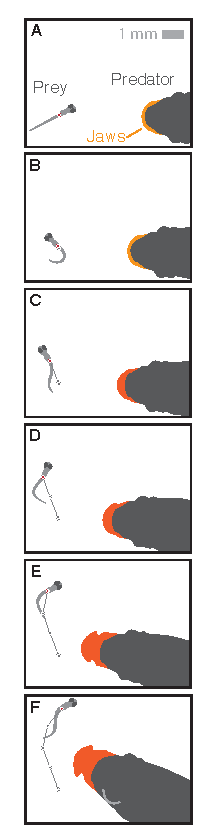
\includegraphics[width=.35\textwidth]{Fig_01.pdf}
\centering	
\caption{\textbf{A predator-prey interaction in zebrafish.} Silhouettes of zebrafish from a dorsal perspective have been traced from video stills (5 ms interval) as an adult attempts to capture a larva with a suction feeding strike.  (\textbf{A}--\textbf{B}) On the predator's approach, the prey initiates a `fast-start' escape response to accelerate away from the predator. The strike has yet to begin, as shown by the lack of protrusion by the jaws of the predator (orange). (\textbf{C}--\textbf{D}) The predator initiates a strike, which is visible from jaw protrusion (red). (\textbf{E}--\textbf{F})  With its jaws fully extended, the predator fails to capture the prey which proceeds to move away from the predator with rapid undulatory swimming. Recording from \cite{Stewart:2014cm}.}
\label{pred_prey}
\end{SCfigure}

%TODO: Add legend from wainwright review

% FIG 2
\pagebreak
\begin{figure}[t]
\begin{centering}
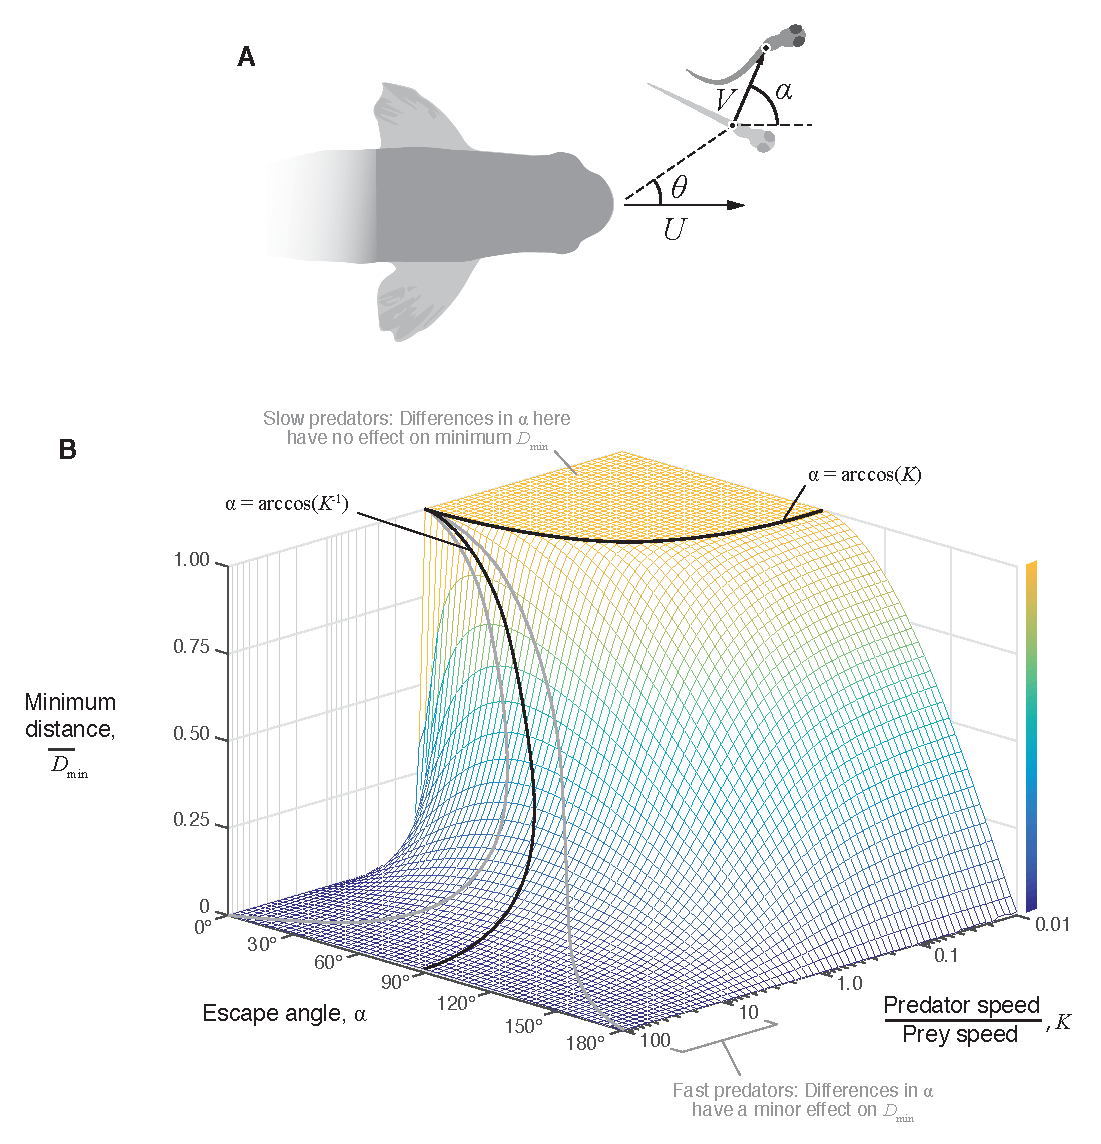
\includegraphics[width=1\textwidth]{Fig_02.pdf}
\centering	
\caption{\textbf{A pursuit model for predator-prey interactions in fish.} (\textbf{A}) Pursuit models consider the motion of a predator (viewed from dorsal perspective) with speed $U$ and a prey with speed $V$ and escape angle $\alpha$. Some versions of this model consider prey positioned lateral to the predator's approach ($\theta_0>0$).  (\textbf{B}) Numerical simulations were run at varying escape angle and predator approach speed to examine variation in the minimum distance. At $K>1$, the optimal angle (black curve) was predicted analytically (Eqn. ref{K>1} by \cite{Weihs:1984jq}. Deviation from the optimum by $0.1\ol D_{\text{min}}$ (gray curves) is shown to increase at greater values of $K$. The performance plateau where $D_{\text{min}}=1$ is predicted by Eqn. \ref{anglerange}.}

\label{weihs_topo}
\end{centering}
\end{figure}

%TODO: Change D_min*


% FIG 3
\pagebreak
\begin{figure}[t]
\begin{centering}
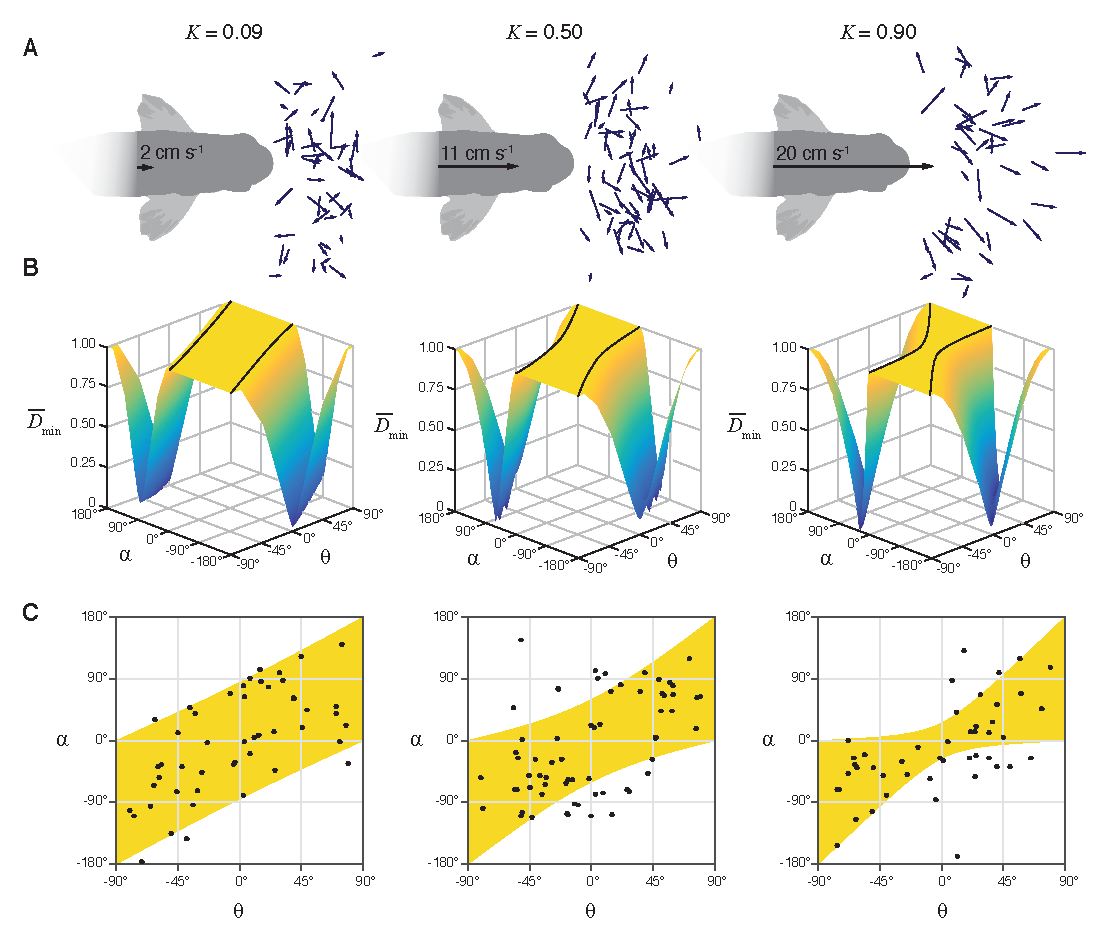
\includegraphics[width=1\textwidth]{Fig_03.pdf}
\centering	
\caption{\textbf{Model predictions and measurements of the fast start.} \textbf{(A)}  }
\label{our_topo}
\end{centering}
\end{figure}

%TODO: unitalicize the "min" in "Dmin"

% FIG 4
\pagebreak
\begin{figure}[t] 
\begin{centering}
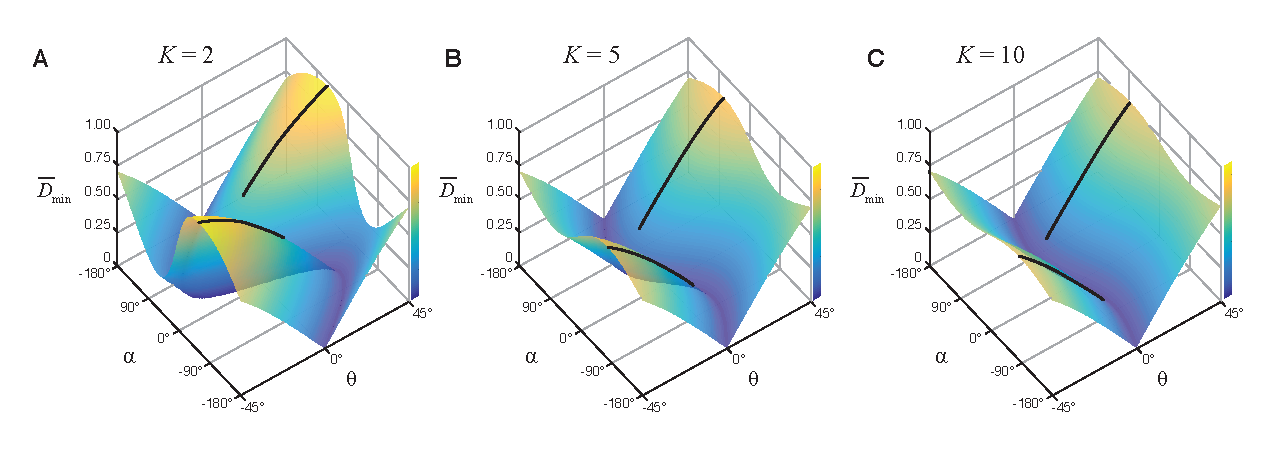
\includegraphics[width=1.1\textwidth]{Fig_04.pdf}
\centering	
\caption{\textbf{Title.} \textbf{(A)}  }
\label{k>1_topo}
\end{centering}
\end{figure}






% CLOSE DOCUMENT
\end{document}
